%%%%%%%%%%%%%%%%%%%%%%%%%%%%%%%%%%%%%%%%%
% Beamer Presentation
% LaTeX Template
% Version 1.0 (10/11/12)
%
% This template has been downloaded from:
% http://www.LaTeXTemplates.com
%
% License:
% CC BY-NC-SA 3.0 (http://creativecommons.org/licenses/by-nc-sa/3.0/)
%
%%%%%%%%%%%%%%%%%%%%%%%%%%%%%%%%%%%%%%%%%

%---------------------------------------------------------------
%	PACKAGES AND THEMES
%---------------------------------------------------------------

\documentclass[unicode]{beamer}

\mode<presentation> {

% The Beamer class comes with a number of default slide themes
% which change the colors and layouts of slides. Below this is a list
% of all the themes, uncomment each in turn to see what they look like.

%\usetheme{default}
%\usetheme{AnnArbor}
%\usetheme{Antibes}
%\usetheme{Bergen}
%\usetheme{Berkeley}
%\usetheme{Berlin}
%\usetheme{Boadilla}
%\usetheme{CambridgeUS}
%\usetheme{Copenhagen}
%\usetheme{Darmstadt}
%\usetheme{Dresden}
%\usetheme{Frankfurt}
%\usetheme{Goettingen}
%\usetheme{Hannover}
%\usetheme{Ilmenau}
%\usetheme{JuanLesPins}
%\usetheme{Luebeck}
\usetheme{Madrid}
%\usetheme{Malmoe}
%\usetheme{Marburg}
%\usetheme{Montpellier}
%\usetheme{PaloAlto}
%\usetheme{Pittsburgh}
%\usetheme{Rochester}
%\usetheme{Singapore}
%\usetheme{Szeged}
%\usetheme{Warsaw}

% As well as themes, the Beamer class has a number of color themes
% for any slide theme. Uncomment each of these in turn to see how it
% changes the colors of your current slide theme.

%\usecolortheme{albatross}
%\usecolortheme{beaver}
%\usecolortheme{beetle}
%\usecolortheme{crane}
%\usecolortheme{dolphin}
%\usecolortheme{dove}
%\usecolortheme{fly}
%\usecolortheme{lily}
%\usecolortheme{orchid}
%\usecolortheme{rose}
%\usecolortheme{seagull}
%\usecolortheme{seahorse}
%\usecolortheme{whale}
%\usecolortheme{wolverine}

%\setbeamertemplate{footline} % To remove the footer line in all slides uncomment this line
%\setbeamertemplate{footline}[page number] % To replace the footer line in all slides with a simple slide count uncomment this line

%\setbeamertemplate{navigation symbols}{} % To remove the navigation symbols from the bottom of all slides uncomment this line

}

\usepackage{amsmath}
\usepackage{amssymb}
\usepackage{booktabs} % Allows the use of \toprule, \midrule and \bottomrule in tables
\usepackage{hyperref}
\usepackage{graphicx} % Allows including images
\usepackage{multirow}
\usepackage[russian]{babel}
\usepackage[utf8]{inputenc}

\setbeamertemplate{footnote}{\noindent\raggedright\insertfootnotetext\par}

%-----------------------------------------------------------------
%	TITLE PAGE
%-----------------------------------------------------------------

\title[]{Методы повышения разнообразия в системах машинного перевода}

\author{Михаил Солоткий}
\institute[ФКН ВШЭ] % Your institution as it will appear on the bottom of every slide, may be shorthand to save space
{
    НИУ Высшая Школа Экономики \\
    Факультет компьютерных наук \\
    Базовая кафедра Яндекса \\
    \bigskip
    {\bf Курсовая работа} \\
    \bigskip
    %Научный руководитель --- Алексей Носков, Яндекс \\
    %Научный консультант --- Сергей Губанов, Яндекс
    Научный руководитель --- Бабенко Максим Александрович
    \bigskip
}
\date{Москва 2020 г.} % Date, can be changed to a custom date

\begin{document}

\begin{frame}
\titlepage % Print the title page as the first slide
\end{frame}

%----------------------------------------------------------------
%	PRESENTATION SLIDES
%----------------------------------------------------------------

%------------------------------------------------
\section{Постановка задачи}
%------------------------------------------------

\subsection{Введение}
\begin{frame}
\frametitle{Цели и задачи}
\begin{itemize}
    \item Обычно системы машинного перевода по одному предложению выдают одно предложение \newline
    \item Цель: построить метод, генерирующий несколько разнообразных переводов \newline
    \item Цель: максимизировать разнообразие и качество \newline
\end{itemize}
\end{frame}

\subsection{Введение}
\begin{frame}
\frametitle{Мотивация}
\begin{itemize}
    \item Цели пользователя неизвестны \newline
    \item Помощь в изучении языка \newline
    \item Генерация переводов разного стиля \newline
\end{itemize}
\end{frame}


\subsection{Нейросетевой машинный перевод}
\begin{frame}
\frametitle{Нейросетевой машинный перевод}
\begin{center}
    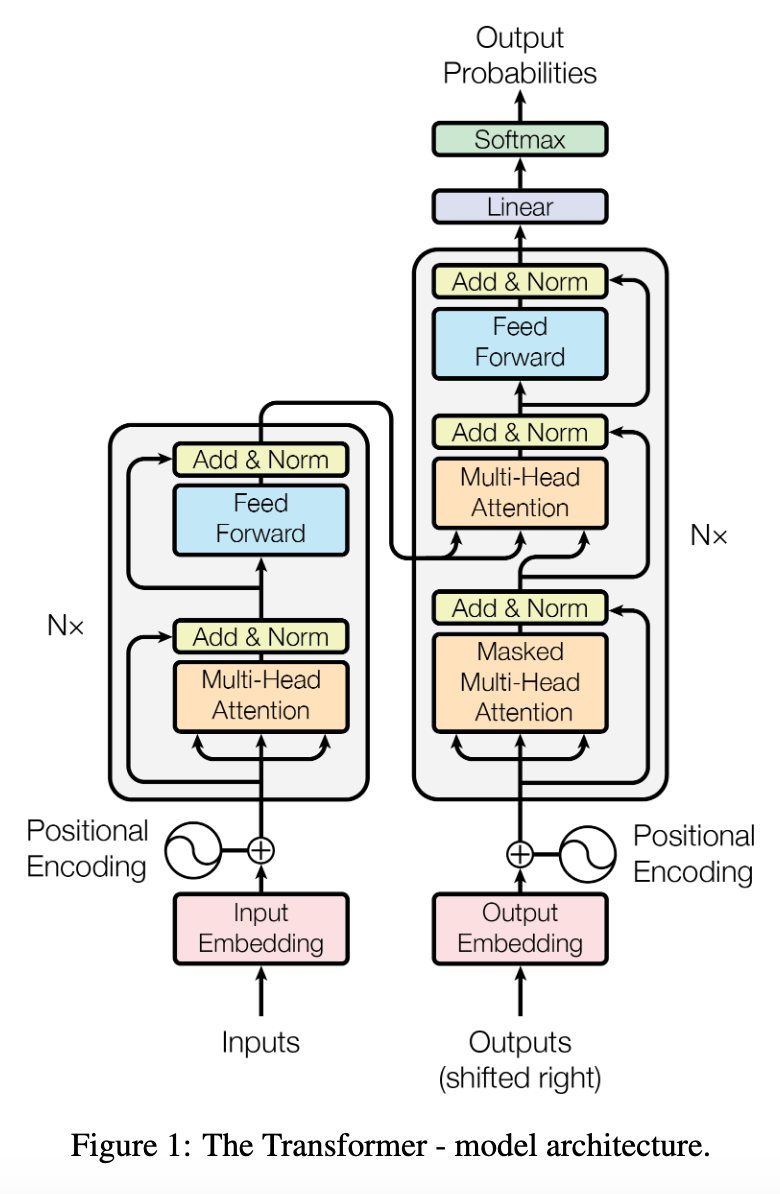
\includegraphics[scale=0.2]{transformer}
\end{center}

\begin{itemize}
    \item $p \, (\bold{y}  |  \bold{x}) = \prod\limits_{t=1}^n \, p \, (y_t | \, \bold{y}_{< t}, \bold{x} ) \rightarrow \max\limits_{\bold{y}}$
    \item beam search выдаёт $k$ приближённо наиболее вероятных переводов
    \footnotetext{Vaswani, A. et al (2017). Attention is all you need. Advances in Neural Information Processing Systems}
\end{itemize}
\end{frame}


\subsection{Данные}
\begin{frame}
\frametitle{Данные}
\begin{itemize}
    \item Обучение на закрытых данных \newline
    \item Тестировалось на WMT'18 en-ru
\end{itemize}
\end{frame}


\subsection{BLEU}
\begin{frame}
\frametitle{BLEU}
\begin{itemize}
    \item $\textrm{BLEU}(out, ref) = \min \Bigg\{ 1, \exp \Big\{ \frac{\textrm{len}(ref)}{\textrm{len}(out)} \Big\} \Bigg\} \Big[ \prod\limits_{i=1}^4 \textrm{precision}_i \Big]^{\frac{1}{4}}$ \newline
    \item Не учитывает смысл перевода, а только совпадение n-грамм
\end{itemize}

\footnotetext{Papineni, K. et al (2002). Bleu: a method for automatic evaluation of machine translation. Association for Computational Linguistics}
\footnotetext{Sulem, E., et al (2018). BLEU is not suitable for the evaluation of text simplification. Association for Computational Linguistics.}
\end{frame}


\subsection{Метрики качества и разнообразия}
\begin{frame}
\frametitle{Метрики качества и разнообразия}
\begin{itemize}
    \item avg-BLEU \newline
    \item max-BLEU \newline
    \item min-BLEU \newline
    \item $\textrm{self-BLEU}(outs) = \frac{1}{\textrm{len} \, (outs) \, ^2} \sum\limits_{i=1}^m \sum\limits_{j=1}^m \textrm{BLEU} (outs_i, outs_j )$ \newline
    \item $\textrm{diversity}(outs) = 1 - \textrm{self-BLEU}(outs)$ \newline
    \item Некорректно сравнивать при разном числе переводов \newline
    \item Фиксируем число переводов, k =3
\end{itemize}
\end{frame}


\subsection{Temperature sampling}
\begin{frame}
\frametitle{Temperature sampling}
$$\textrm{softmax}_i(\bold{z}; t) = \textrm{softmax}_i \Big( \frac{\bold{z}}{t} \Big) = \frac{\exp(z_i \, / \, t)}{\sum\limits_{j=1}^n \exp(z_j \, / \, t)}$$
    \begin{center}
        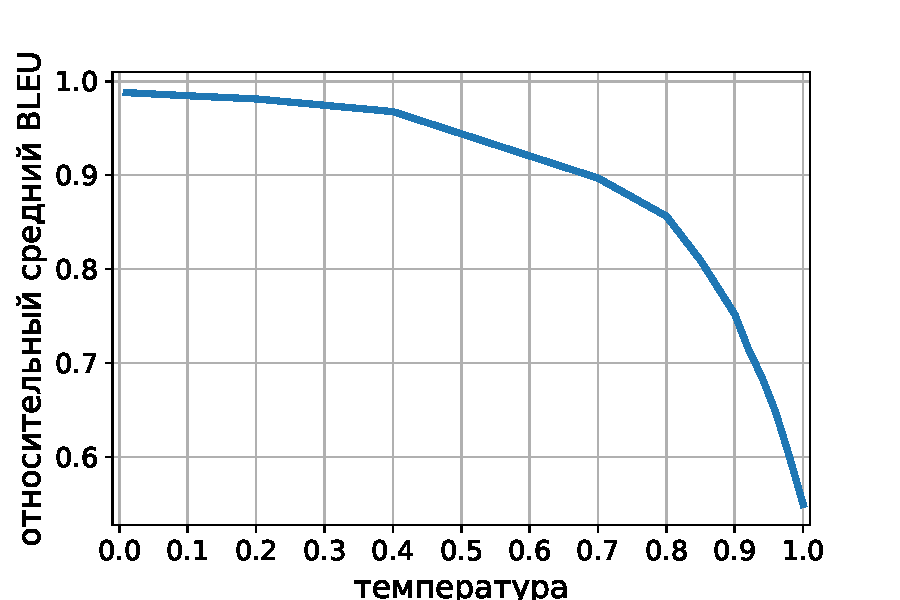
\includegraphics[scale=0.25]{avg-bleu-temperature-sampling.pdf}
        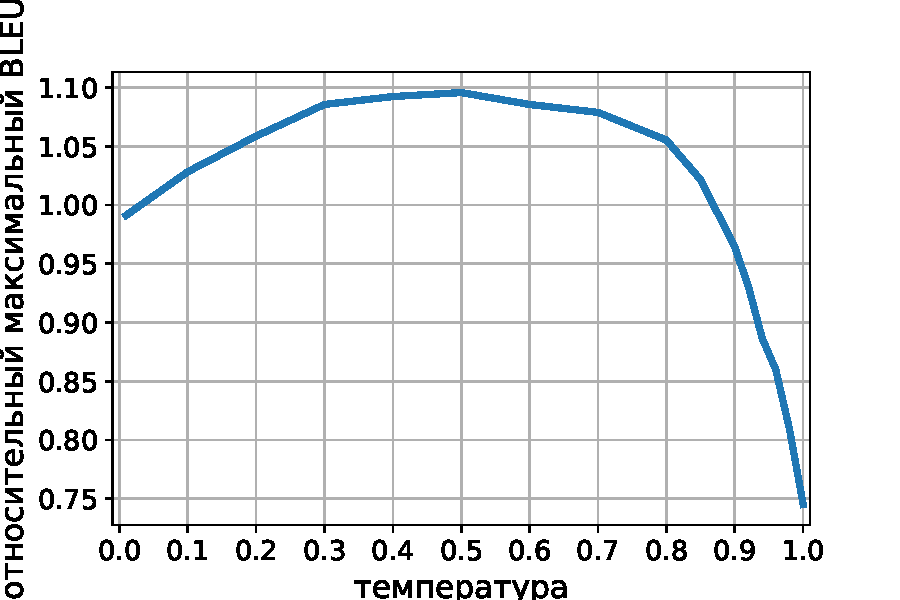
\includegraphics[scale=0.25]{max-bleu-temperature-sampling.pdf}
    \end{center}

    \begin{center}
        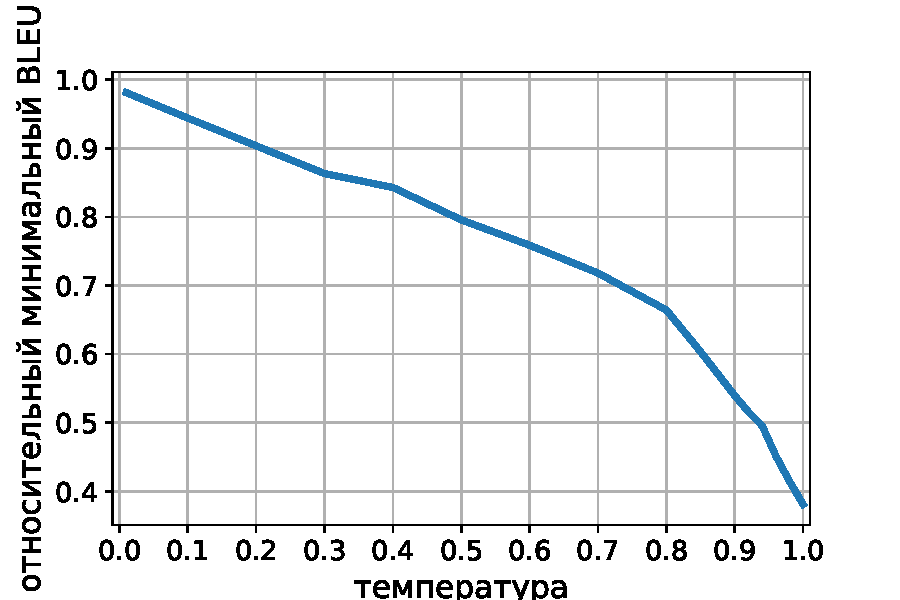
\includegraphics[scale=0.25]{min-bleu-temperature-sampling.pdf}
        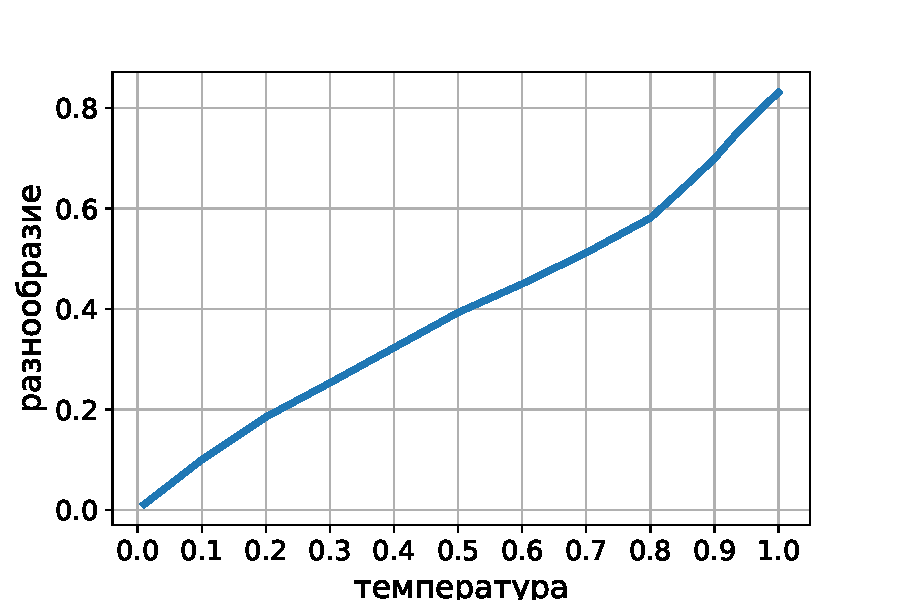
\includegraphics[scale=0.25]{diversity-temperature-sampling.pdf}
    \end{center}
\end{frame}


\subsection{Nucleus sampling}
\begin{frame}
\frametitle{Nucleus sampling}
\begin{itemize}
    \item Отбросить $p$ вероятностной массы, приходящейся на токены с самой низкой вероятностью и взять семпл
\end{itemize}
\begin{center}
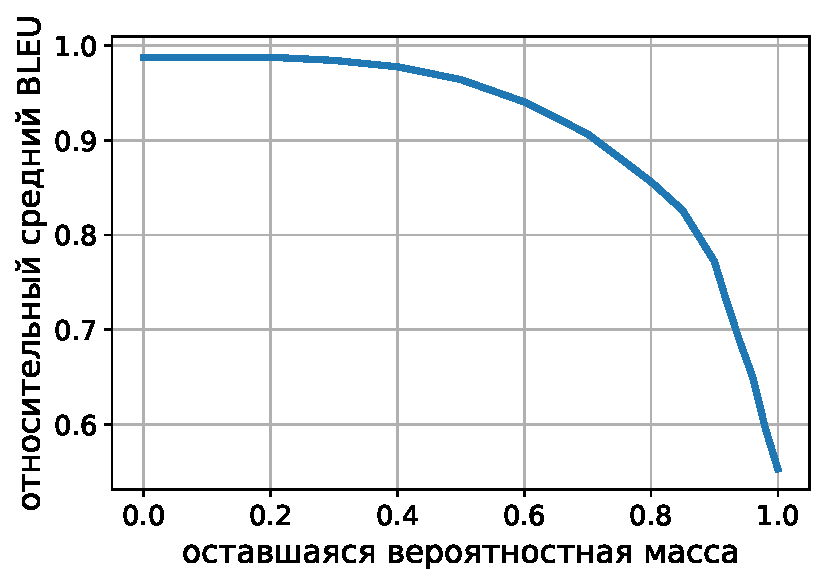
\includegraphics[scale=0.25]{avg-bleu-nucleus-sampling.pdf}
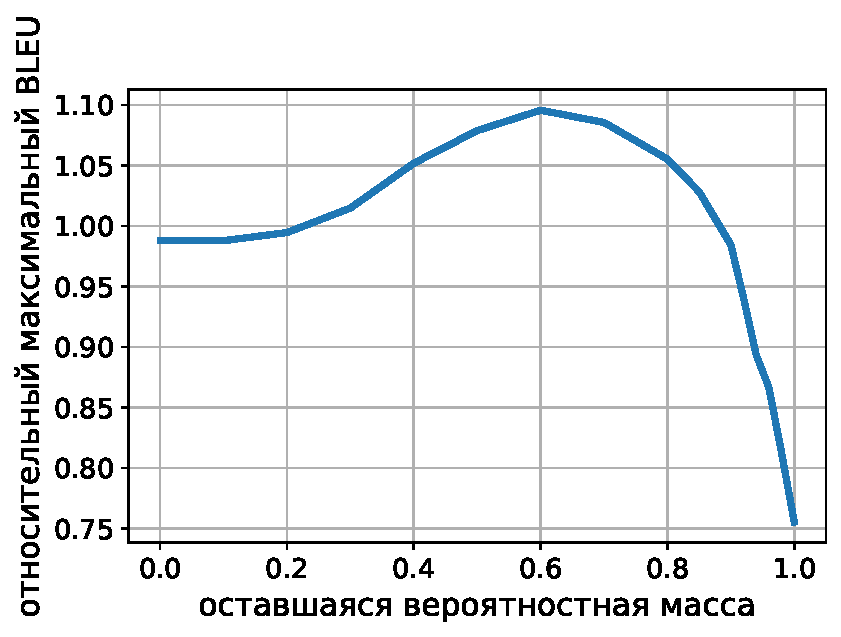
\includegraphics[scale=0.25]{max-bleu-nucleus-sampling.pdf}
\end{center}

\begin{center}
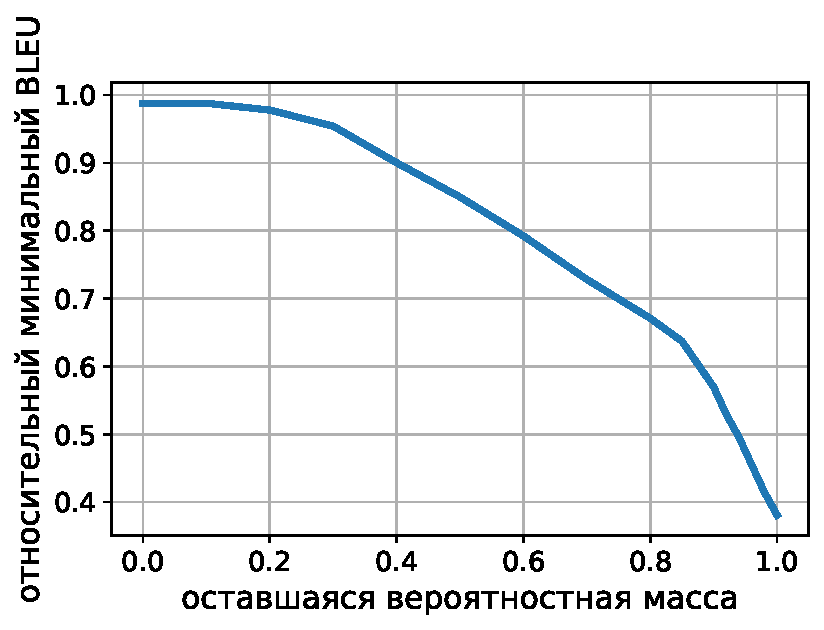
\includegraphics[scale=0.25]{min-bleu-nucleus-sampling.pdf}
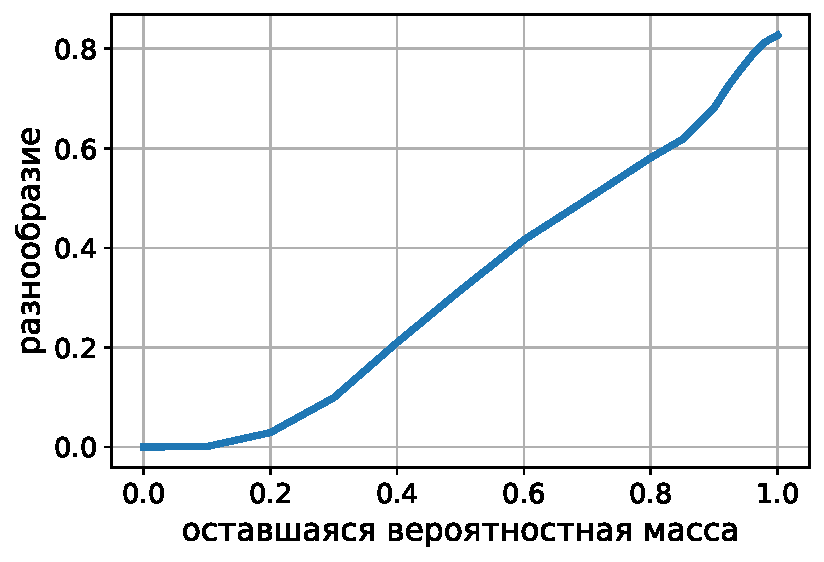
\includegraphics[scale=0.25]{diversity-nucleus-sampling.pdf}
\end{center}
\footnotetext{Holtzman, A. et al (2019). The curious case of neural text degeneration.}
\end{frame}


\subsection{Другие идеи}
\begin{frame}
\frametitle{Другие идеи}
\begin{itemize}
    \item Diverse Resampling: семплируем 10 переводов, из них выбираем наиболее разнообразные \newline
    \item Модель с латентными переменными: к сети добавляется автокодировщик, энкодер и декодер в процессе перевода обуславливаются на семплируемые латентные переменные
\end{itemize}
\end{frame}


\subsection{Diverse Beam Search}
\begin{frame}
\frametitle{Diverse Beam Search}
$$\ln p \, (y_t \, | \, \bold{y}_{<t}, \bold{x}) + \sum_{i=1}^{k - 1} \lambda_i \, \textrm{div}(\bold{y}_{\leq t}, \, \bold{y}^i) \rightarrow \max\limits_{y_t}$$
\begin{itemize}
    \item $\lambda_i$ можно брать одинаковыми
    \item есть параллельная версия, которая чуть хуже по качеству последовательной
\end{itemize}

\footnotetext{Vijayakumar, A. K. et al (2016). Diverse beam search: Decoding diverse solutions from neural sequence models.}

\begin{center}
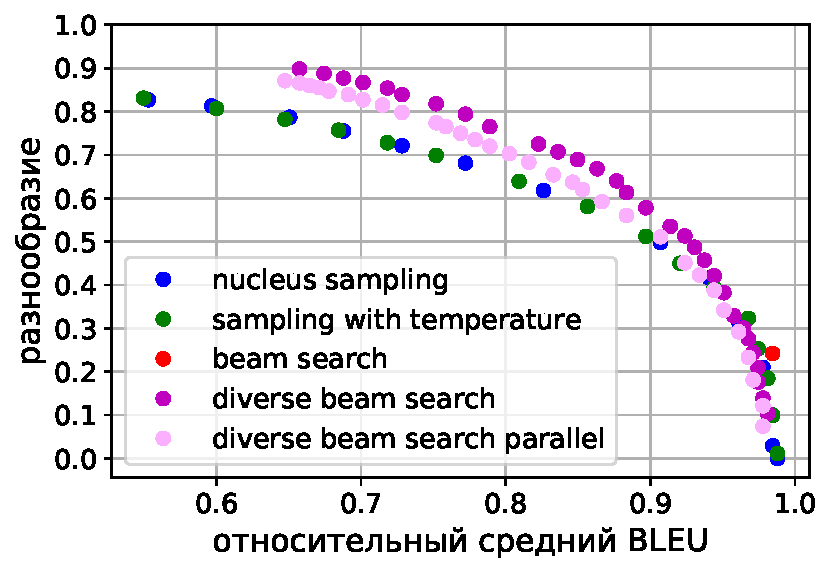
\includegraphics[scale=0.25]{avg-bleu-diverse-beam-search.pdf}
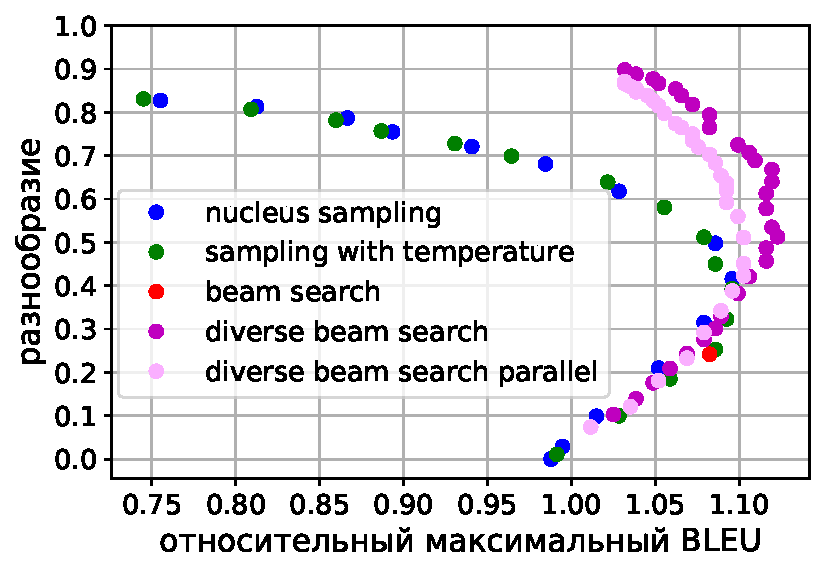
\includegraphics[scale=0.25]{max-bleu-diverse-beam-search.pdf}
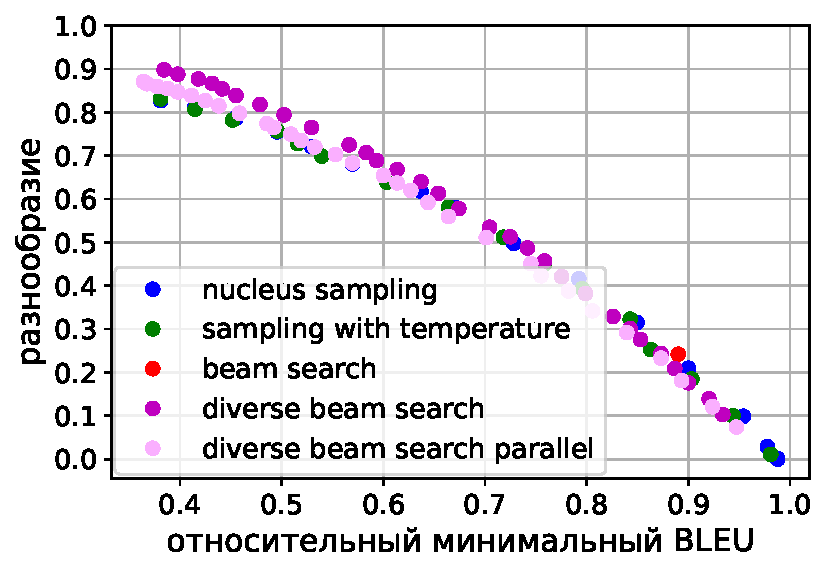
\includegraphics[scale=0.25]{min-bleu-diverse-beam-search.pdf}
\end{center}

\end{frame}


\subsection{Примеры переводов}
\begin{frame}
\frametitle{Примеры переводов}
{\small
Исходное предложение: <<As a coach, I would tell you it's time to run another play.>> \newline

Обычный beam search выдаёт:\\
1) Как тренер, я бы сказал вам, что пришло время запустить другую игру.\\
2) Как тренер, я бы сказал вам, что пришло время запустить еще одну игру.\\
3) Как тренер, я хотел бы сказать вам, что пришло время запустить другую игру.
\newline

Семплинг с температурой t = 0.5 даёт: \\
1) Как тренер, я скажу вам, что пришло время снова сыграть.\\
2) Как тренер, я хотел бы сказать вам, что пришло время провести еще одну игру.\\
3) Как тренер, я бы сказал, что пришло время играть в другой пьесе. \newline

Diverse beam search, $\lambda = 10.0$ переводит так: \\
1) Как тренер, я бы сказал вам, что пришло время запустить другую игру.\\
2) Как тренер, скажу тебе, что пора начать новую игру.\\
3) Как тренер, я хочу сказать, что пришло время начать новую игру.
\newline
}
\end{frame}


\subsection{Результаты}
\begin{frame}
\frametitle{Результаты}
\begin{itemize}
\item Была введена формализация понятий качества и разнообразия в машинном переводе и показана их адекватность \newline
\item Реализованы и испробованы различные методы генерации разнообразных переводов, в том числе придуманы новые \newline
\item Сделано сравнение методов по качеству и разнообразию, а также с точки зрения потребления ресурсов \newline
\item Для лучшего метода -- diverse beam search -- предложена параллельная реализация и адаптация к специально выбранной метрике разнообразия \newline
\end{itemize}
\end{frame}

\subsection{Возможные вопросы}
\begin{frame}
\frametitle{Возможные вопросы}
\begin{itemize}
    \item Как меняются графики при смене домена? \newline
    \item Как это использовать в production, когда нам нужен строго определённый уровень разнообразия? \newline
    \item Какие минусы у diverse beam search и можно ли не использовать семплинг вообще, если есть метод лучше? \newline
    \item Можно ли одновременно сделать идеальными качество и разнообразие? \newline
    \item В чём принципиальная проблема с diverse resampling? \newline
    \item Насколько примеры переводов отражают качество методов и не подобраны ли они специально?
\end{itemize}
\end{frame}


\end{document}